\documentclass[border=10pt]{standalone}

\usepackage{pgfplots}
\usepackage{tikz}
\usepackage{tikzducks}
\pgfplotsset{compat=1.8}
\usepgfplotslibrary{fillbetween} %for fill under curve

\renewcommand{\vec}[1]{\textbf{#1}}

\newcommand{\image}{
	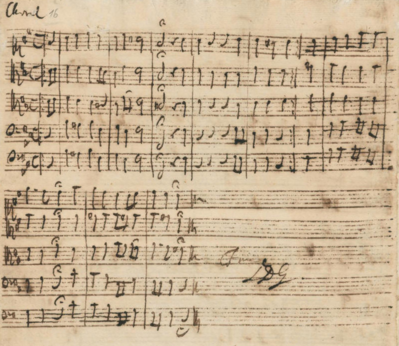
\includegraphics[height=2.3cm]{bach.png}
}
\newcommand{\noise}{
	
\includegraphics[height=2.3cm]{noise.png}
}

\begin{document}

    \begin{tikzpicture}[node distance=2cm, thick, shorten <= 0.3em, shorten >= 0.3em, minimum height=1cm]
		\node[draw, circle, fill=black!30] (T) {$\vec{x}_T$};
		\node[right of=T] (dots1) {$\cdots$};
		\node[draw, circle, right of=dots1, fill=black!20] (t) {$\vec{x}_t$};
		\node[draw, circle, right of=t, node distance=3cm, fill=black!10] (t-1) {$\vec{x}_{t-1}$};
		\node[right of=t-1] (dots2) {$\cdots$};
		\node[draw, circle, right of=dots2] (0) {$\vec{x}_{0}$};
		
		\draw[->] (T) -- (dots1);
		\draw[->] (dots1) -- (t);
		\draw[->] (t) -- node[below] {$p_\theta(\vec{x}_{t-1}|\vec{x}_t)$} (t-1);
		\draw[->, dashed] (t-1) edge[bend right] node[above] {$q(\vec{x}_t|\vec{x}_{t-1})$} (t);
		\draw[->] (t-1) -- (dots2);
		\draw[->] (dots2) -- (0);
		
		\node[minimum height=2cm, below of=T] {\image};
		\node[opacity=1, below of=T] {\noise};
		\node[minimum height=2cm, below of=t] {\image};
		\node[opacity=0.65, below of=t] {\noise};
		\node[minimum height=2cm, below of=t-1] {\image};
		\node[opacity=0.35, below of=t-1] {\noise};
		\node[minimum height=2cm, below of=0] {\image};
    \end{tikzpicture}

\end{document}
